%----------------------------------------------------------------------------
\chapter{Implementáció}
%----------------------------------------------------------------------------

Az elkészült program \emph{Visual Studioban} egy \emph{solutionből}, azon belül két projektből áll. Az egyik projekt a \emph{TSL} fájlt tartalmazza, ez felel az adatbázis felépítéséért, a másik pedig a \Csh{} forrásfájlokat, ez az adatbázis szempontjából a kliensoldalt valósítja meg. A fejlesztést nagyban megkönnyítette, hogy ilyen esetben egyetlen kattintással tudjuk fordítani a két projektet. A továbbiakban először a \emph{TSL} projekt, majd a \emph{Trainbenchmark} nevű \Csh{} fájlokat tartalmazó projekt kerül bemutatásra.

\section{\emph{TrainBenchmarkTSLProject}}

A projekt egyetlen \emph{.tsl} kiterjesztésű fájlból áll. Ez tartalmazza a Train Benchmark modelljének a Graph Engine-ben megfelelő leírását néhány módosítással. A modellben két osztály közötti kapcsolat a gráfban lévő éleket határozzák meg. Az osztályok a gráf csúcsai lesznek. A \emph{TSL} nem támogatja az öröklést, így azokhoz az osztályokhoz, amik öröklődnek fel van véve a szülő összes tulajdonsága. Ez a \emph{Segment} és a \emph{Switch} esetében lényeges, amik a \emph{TrackElement} osztályból öröklődnek, ezért mindkettő tartalmaz \emph{connectsTo} listát.

A Graph Engine-ben a kapcsolatok nem típusfüggőek, minden gráfél \emph{CellId} típussal mutat egy cellára. Ez nagy könnyedség, hiszen amennyiben nem így lenne, azaz meg kéne határozni, hogy egy él milyen osztályú cellára mutat, akkor a \emph{TrackElement} \emph{connectsTo} éleit nem lehetne megvalósítani, ugyanis egy \emph{Segment} élen keresztül csatlakozhat \emph{Switch}-hez és egy másik \emph{Segment}-hez is.

A módosított modell a \ref{fig:GraphEngineTSLModel} ábrán látható. A különbségek, amik ez a modell és a Train Benchmark eredeti modellje között van, az csak az öröklés miatti \emph{connectsTo} élekben van, így a két modell matematikai szempontból ekvivalens.

Az éleknek két fajtája van. Sima \emph{CellId} típusú élek egy-egy kapcsolatot jelölnek, míg a \texttt{List<CellId>} egy-több kapcsolat leírására szolgál. Ez azt jelenti, hogy egy csúcsból egy éltípussal egy másik típusú csúcsba egy él vezet vagy vezethet több másik típusú csúcsba is egy-egy él.

A \texttt{Position}, illetve \texttt{Signal} felsorolásokat is a \emph{TSL} fájlban érdemes leírni, így a gráf csúcsaiban már tárolva vannak.

\begin{figure}[H]
	\centering
	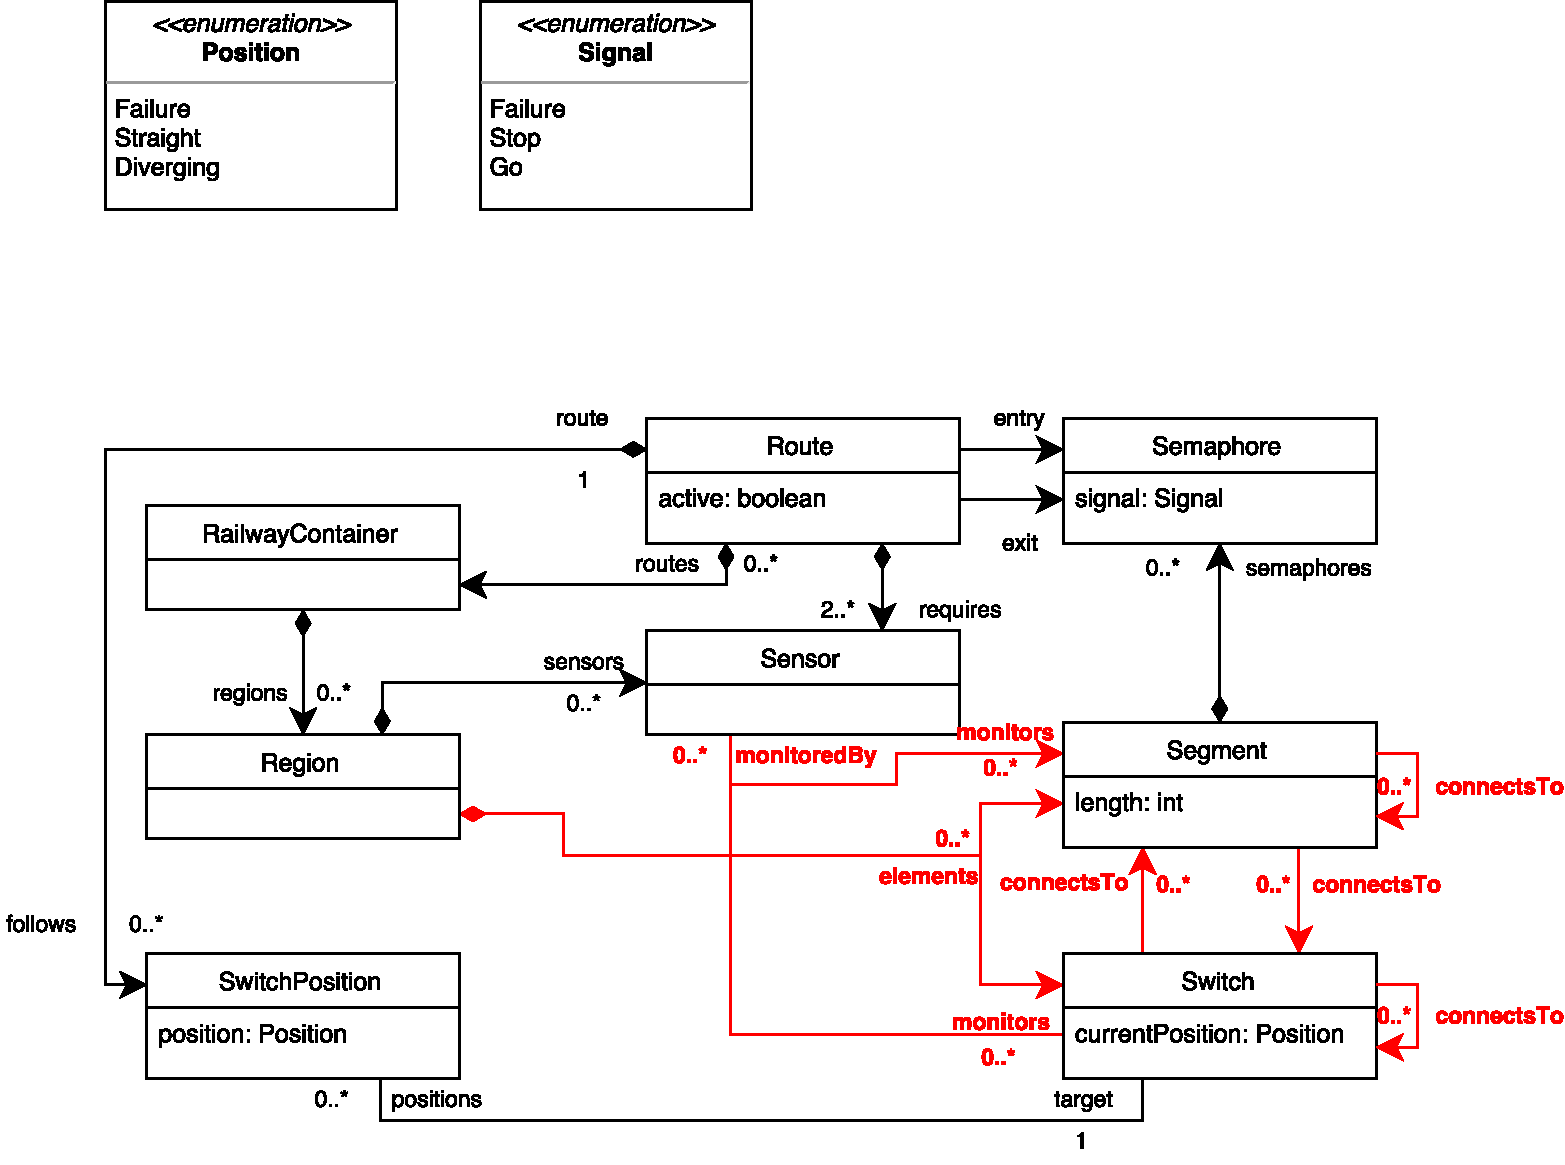
\includegraphics[width=\linewidth, keepaspectratio]{figures/GraphEngineTSLModel.pdf}
	\caption{A \emph{TSL} modell felépítése.}
	\label{fig:GraphEngineTSLModel}
\end{figure}

\section{\emph{\Csh{} project}}

A projekt 7 forrásfájlból és 41 függőségből (\emph{Reference}) épül fel. A függőségek között megtalálható a \emph{TSL} projekt. A Graph Engine használata egy projekten belül globális, így minden osztály és függvény ugyanazokon az adatokon dolgozik.

\subsection{A program belépési pontja}

A \texttt{Program.cs}-ben megtalálható \texttt{Main} függvény a program belépési pontja. Ebben található néhány alapvető konfiguráció, melyeknek két fő célja van.
\begin{itemize}
	\item A futási idő méréséhez a futtató folyamatot a 2-es processzormagon van futtatva, mert a háttérben futó folyamatok és szolgáltatások jelentős része az 1-es számú processzormagot használja. Így nagyobb eséllyel fut a program tisztább környezetben.
	\item A Graph Engine motorja lokális futásra van konfigurálva, ezáltal nem használ hálózati erőforrást, nincs a lekérdezéseknek felesleges \emph{overhead}-je.
\end{itemize}

Itt található még egy iteráció, mely végigmegy az előre elkészített modelleken méret szerint, és mindegyik méretre végrehajtatja a mérést. A mérés lépései a \texttt{Test.cs} fájlban találhatóak. Minden mérés három lépésből (beolvasás, validáció, módosítás) áll. Egy lépésben a program végrehajtja a modellen a megfelelő műveletet, és az ezalatt eltelt időt tároljuk el.

\subsection{Beolvasás}

A beolvasás a modell \emph{.ttl} fájlból való feldolgozását, majd az adatbázisba való mentését jelenti. Az \emph{RDFReader} osztály \texttt{read()} metódusa valósítja meg. A \emph{.ttl} fájl \emph{Turtle} formátumot takar. Ez egy olyan fájltípus, mely alkalmas az \emph{RDF} típusú gráfok tárolására. 

Több olyan könyvtár létezik a .Net-hez, ami \emph{Turtle} típusú fájlokat tud feldolgozni. Ezek közül a \emph{dotNetRDF} nevű ingyenes és nyílt forráskódú könyvtárat használja a program. Ennek kezelése egyszerű, jól átlátható. A \emph{Turtle} állományban található \emph{Triple}-öket beolvassa a memóriába és készít egy gráfot, amit már gyorsan be lehet járni. Az elkészült gráf bejárása a következőképpen zajlik:

\begin{itemize}
	\item Kiválasztjuk egy listába azokat a \emph{Triple}-öket, melyek a csúcsok típusát írják le.
	\item Végigiterálunk a listán és minden csúcshoz létrehozunk egy megfelelő típusú osztályt.
	\item Megkeressük azokat a további \emph{Triple}-öket, melyek az adott csúcshoz tartoznak és a hozzá kapcsolódó tulajdonságokat, éleket tárolják, majd ezeket az információkat beleírjuk az osztályunkba.
	\item Az elkészült osztályt elmentjük a Graph Engine adatbázisába.
\end{itemize}

A feldolgozás folyamán két konverzióra van szükség, mégpedig azért, mert a \emph{Turtle} fájlban egyszerű szövegként van tárolva a \emph{Signal} és a \emph{Position}. Ezeket \emph{enum}-má kell konvertálni, hogy a Graph Engine csúcsaiba tulajdonságként el tudjuk menteni.

\subsection{Validáció}

Ebben a lépésben a modell ellenőrzése következik. Mindkét kényszer esetén fontos az is, hogy a modellben hol sérülnek, mivel egy valós fejlesztési folyamat során is fontos, hogy a tervező ki tudja javítani a problémákat és ezt csak úgy tudja megtenni, ha tudja, hogy hol vannak. Így egyik esetben sem elég megtalálni az első olyan pontot a modellben, ahol a kényszer nem teljesül. Ez a programban úgy lett megvalósítva, hogy bejárja az egész modellt és összeszámolja a hibás helyeket.

A modellvalidációs osztály a \emph{Validator} nevet viseli. Két függvényből áll, melyek a \texttt{SwitchSet()} és a \texttt{RouteSensor()}, a két megvalósított kényszer neve alapján. Mindkét függvény egy egész számot ad eredményül, ami azon elemek számát jelöli, melyek nem felelnek meg a követelményeknek. 

\subsubsection{\emph{SwitchSet}}

A \emph{SwitchSet} kényszer ellenőrzéséhez az összes modellben szereplő \emph{Route}-on, melynek kezdetén a \emph{Semaphore} \emph{Signal}-ja \emph{Go} értékű, lévő \emph{SwitchPosition} és a hozzátartozó \emph{Switch} \emph{Position} tulajdonsága meg kell egyezzen. Ezért a függvényben először a \emph{Semaphore}-okon iterálunk végig, majd azokon az utakon, melyeknek kezdőpontja az adott \emph{Semaphore}, végül pedig a hozzá tartozó \emph{SwitchPosition} és az ahhoz tartozó \emph{Switch} tulajdonságait kérjük le. A folyamat forráskódja a ábrán látható.
%TODO ábra

Több típusú csúcson kell műveleteket végezni, ezáltal a \emph{LINQ}-es lekérdezések eredményét használat előtt el kell tárolni egy lokális változóban a \texttt{ToList()} függvény segítségével. Enélkül a \ref{graphenginelinq} fejezetben tárgyalt okok miatt holtpont alakulna ki. Az egymás utáni \texttt{using} blokkok használatánál is ugyanilyen módszerrel el kell tárolnunk az adott változó értékét.

\subsection{Módosítás és újraellenőrzés}

A modellen történő módosításokat a \emph{Modifier} osztály végzi. Négy különböző eset van, az alapján, hogy a \emph{SwitchSet} vagy a \emph{RouteSensor} kényszer kapcsán történik a módosítás, illetve \emph{Inject} vagy \emph{Repair} a célja. A modell elrontása egyszerűbb művelet a javításnál, ugyanis nem kell hibát keresni és azt kijavítani, elég csak megkeresni egy elemet és a megfelelő értékét hibásra állítani. Ezt követi az újraellenőrzés, ami a validációs szakasz ismételt futtatását jelenti. A módosítás és az újraellenőrzés ilyen sorrendben egymás után többször végrehajtódik.

\subsection{Mérés és az eredmények elmentése}

Minden szakasz futási ideje a \emph{System.Diagnostic.StopWatch} osztály segítségével lett lemérve. A Train Benchmark többi \emph{Tool}-ja $ns$-ban ad eredményt a futás idejéről, azonban két azonos konfigurációjú , egymás után történő futtatás eredménye is legalább 100 $\mu{}s$-mal eltér. Ezen megfontolás miatt az elkészült program futásidő-mérésének pontossága 1 $\mu{}$s. A \emph{StopWatch} osztályban az \texttt{ElapsedTicks} és a \texttt{Frequency} \emph{property}-k segítségével lehet $ms$-nál pontosabb eredményt elérni. 

\section{Többi \emph{Tool} futtatása}
